\newpage
\section{Modelos de Casos de Uso}
\subsection{Modelo de Casos de Uso de alto nível}
Diagrama geral de Use Cases

\begin{comment}
\begin{figure}[!htb]
	\centering
	\includegraphics[scale=0.85]{images/diagramaGeralDeUseCase}
	\caption {Diagrama geral de \emph{Use Cases} do produto}
\end{figure}
\end{comment}

\subsection{Modelos de Casos de Uso detalhado}
\subsubsection{\textbf{1 - HoneyPot}}
\begin{itemize}
 \item \textbf{Identificar system calls e actualizar BD} -  Tal como apresentado no diagrama abaixo, o QEMU é capaz de identificar system calls
 do guest OS mais seu contexto. Após detectar uma chamada este actualiza a Base de dados com essa informação. 
 \item \textbf{Copiar ficheiros} - O QEMU pode também copiar qualquer ficheiro do guest OS para o Host OS ou para outro ponto remoto.
 \item \textbf{Filmar HoneyPot} - Mais ainda o QEMU é capaz de capturar uma sequência de capturas de ecrã do que se passa no guest, 
 criando assim um ficheiro em formato vídeo para, mais tarde o utilizador poder ver.
 \end{itemize}

\begin{figure}[!ht]
	\centering
	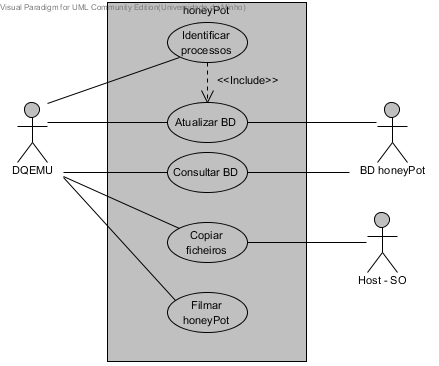
\includegraphics[scale=0.80]{images/ucs/HoneyPot}
	\caption {Diagrama de use case, parte do HoneyPot}
\end{figure}
\pagebreak

\subsubsection{\textbf{2 - Rede}}
\begin{itemize}
 \item \textbf{Captura trâfego} - O Snort e o TShark tem como função capturar todo o tipo de trâfego que passe pela rede. Toda essa informação
 irá convergir para o Delusion Collector Daemon (DCD) que irá registar essa informação na base de dados.
 \item \textbf{Filta trâfego} - O TShark pode adicionalmente filtrar o tráfego que coleta segundo critérios escolhidos pelo utilizador
 \item \textbf{Analisa trâfego} - O Snort irá analisar o tráfego e procurar por padrões de eventos maliciosos, quando encontrar um padrão gera um
 alerta, que será capturado pelo DCD.
 \end{itemize}

\begin{figure}[!ht]
	\centering
	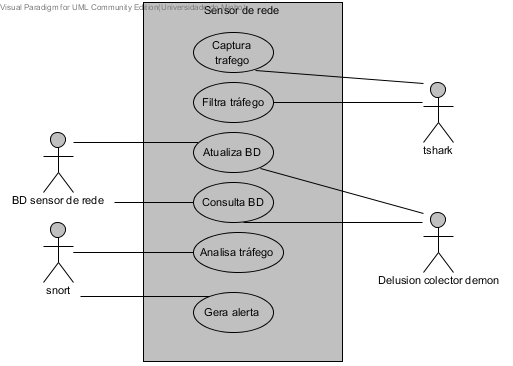
\includegraphics[scale=0.80]{images/ucs/Rede}
	\caption {Diagrama de use case, parte da Rede}
\end{figure}
\pagebreak

\newcommand{\uticomum}{\emph{utilizador comum}\xspace} 
\newcommand{\admini}{\emph{administrador}\xspace} 
\newcommand{\visualz}{\emph{visualizador}\xspace}
\subsubsection{\textbf{3 - Visualizador}}

Como já foi referido anteriormente (sec~\ref{sec: olare}) existem dois tipos de utilizadores: o \uticomum; e o \admini.\\ 

O \admini terá a mesma interacção com o \visualz que o \uticomum tem (que será explicado mais adiante), mais uma responsabilidade acrescida, 
conforme se pode ver na Figura~\ref{fig: casodeusovisual}:

\begin{itemize}
 \item \textbf{Configurar utilizadores} - esta funcionalidade diz respeito à gestão de utilizadores e engloba acções do tipo adicionar/remover utilizadores, 
 alterar permissões (por exemplo: acesso a configurações, tipos de visualizações permitidas, etc). A sua explicação estará mais detalhada em~\ref{subsubsec: confighoney} - 6.
\end{itemize}

O \uticomum terá como interacção com o sistema as seguintes funcionalidades:

\begin{itemize}
 \item \textbf{Ver Tráfego} - a funcionalidade que diz respeito a todas as formas de visualização que serão disponibilizadas pelo \visualz. Maioritariamente, a informação será exibida através de gráficos (de diversos tipos) e tabelas.
 \item \textbf{Ver Alertas} - os alertas que serão processados pelo \visualz, tanto poderão dizer respeito ao \emph{honeypot} como à rede.
 \item \textbf{Aplicar Filtros} - o utilizador poderá aplicar filtros às suas pesquisas, de modo a focalizar a informação ao que realmente lhe interessa.
 \item \textbf{Configurar Rede} - esta funcionalidade diz respeito às configurações que o utilizador poderá fazer à rede. A sua explicação estará mais detalhada em~\ref{subsubsec: confighoney} - 5.
 \item \textbf{Configurar Honeypot} - Finalmente, o utilizador poderá também configurar o \emph{honeypot}. A sua explicação estará mais detalhada em~\ref{subsubsec: confighoney} - 4.
\end{itemize}

\begin{figure}[!ht]
	\centering
	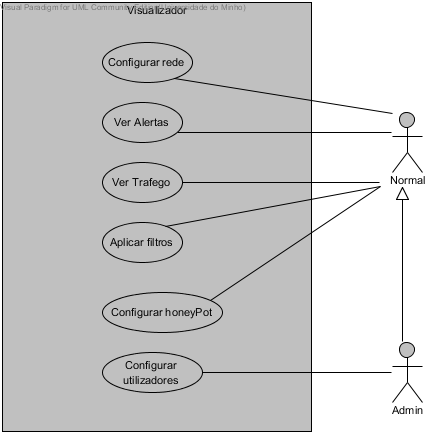
\includegraphics[scale=0.80]{images/ucs/Visualizador}
	\caption {Diagrama de use case, parte da Rede}~\label{fig: casodeusovisual}
\end{figure}
\pagebreak

\subsubsection{\textbf{4 - Configuração HoneyPot}}~\label{subsubsec: confighoney}

Uma das funcionalidades disponíveis na interação utilizador-\visualz, é a configuração do \emph{honeypot} (ver Figura~\ref{fig: confighoney}).
Esta funcionalidade está divida em três acções que o utilizador poderá tomar, sendo essas acções:

\begin{itemize}
 \item \textbf{Indicar SO} - através desta funcionalidade, o utilizador poderá indicar qual o sistema operativo que pretende virtualizar, indicando também certos parâmetros de \emph{hardware} da máquina.
 \item \textbf{Indicar serviços activos} - o utilizador poderá configurar, através do \visualz, quais os serviços activos que o \emph{honeypot} terá. Por exemplo, ter ou não activo um servidor \emph{apache}.
 \item \textbf{Indicar vulnerabilidades} - finalmente, o utilizador poderá também configurar certas vulnerabilidades nos serviços activos do \emph{honeypot}.
\end{itemize}

\begin{figure}[!ht]
	\centering
	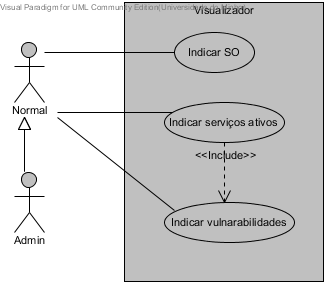
\includegraphics[scale=0.80]{images/ucs/ConfHoneyPot}
	\caption {Diagrama de use case, configuração HoneyPot}~\label{fig: confighoney}
\end{figure}
\pagebreak

\subsubsection{\textbf{5 - Configuração Rede}}
Como se pode ver na Figura~\ref{fig: confrede}, o utilizador poderá, caso tenha permissões para isso, configurar certas ferramentas que actuam sobre a rede. Desse modo, tem-se:

\begin{itemize}
 \item \textbf{Configurar IpTables} - configurar \emph{iptables}, será ...
 \item \textbf{Configurar Snort} - a configuração do \emph{Snort} passa por indicar parâmetros que irão influenciar na captura de pacotes ...
 \item \textbf{Configurar Tshark} - a configuração do \emph{Tshark} permitirá fazer alterações que influenciam o comportamento do mesmo, à semelhança do \emph{Snort}.
 \item \textbf{Configurar Rede} - esta funcionalidade diz respeito aos diversos parâmetros restantes que se podem modificar na rede. Tem-se como exemplo, a configuração de ...
\end{itemize}

\begin{figure}[!ht]
\centering
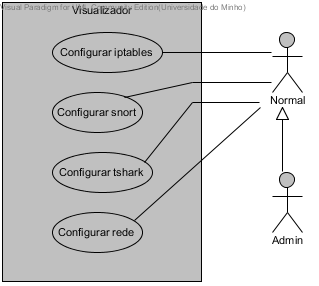
\includegraphics[scale=0.80]{images/ucs/ConfRede}
\caption {Diagrama de use case, configuração Rede}~\label{fig: confrede}.
\end{figure}
\pagebreak

\subsubsection{\textbf{6 - Configuração Utilizadores}}
Como na maioria dos sistemas de \emph{software}, haverá um controlo/gestão de utilizadores por parte de um ou mais \emph{administradores}. Assim, cabe ao \admini fazer essa gestão a partir das seguintes funcionalidades, consoante se pode ver na Figura~\ref{fig: confutil}:

\begin{itemize}
 \item \textbf{Criar Utilizador} - esta acção permite ao \admini criar um utilizador, indicando também certas propriedades que este irá ter, como por exemplo: se será o novo ultizador um \admini ou um \uticomum, se poderá ter permissões para configurar a rede/\emph{honeypot}, etc.
 \item \textbf{Editar Utilizador} - a partir desta acção, o \admini poderá alterar certas propriedade de um utilizador que foram, ou não, definidas aquando a sua criação.
 \item \textbf{Remover Utilizador} - finalmente, o \admini poderá eliminar utilizadores. A eliminação de um utilizador poderá implicar também a eliminação de outros registos.
\end{itemize}

\begin{figure}[!ht]
\centering
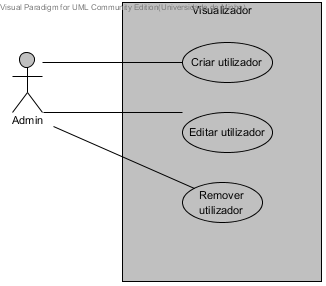
\includegraphics[scale=0.80]{images/ucs/ConfUtilizadores}
\caption {Diagrama de use case, configuração Utilizadores}~\label{fig: confutil}
\end{figure}
\pagebreak

